\hypertarget{00-cover}{}
\hypertarget{bathroom-emergency-guide}{%
\section{Bathroom Emergency Guide}\label{bathroom-emergency-guide}}

\hypertarget{in-case-of-too-much}{%
\subsection{In case of too much}\label{in-case-of-too-much}}

\begin{quote}
You are in a room with a door, water, and one next action.\\
That is enough to begin.
\end{quote}

112life or lasting harm

116 117urgent medical help

116 123a human voice

110police / active threat

\textbf{Version 4.0 · Germany edition · 17 July 2026}

A small decision system for panic, pain, responsibility, danger,
overload, bad smells, missing places, and the occasional collapse of
civilization.

The jokes are optional. The red flags are not.

This guide supports decisions; it does not diagnose, replace first-aid
training, or overrule emergency dispatchers. If life may be in danger or
lasting harm cannot be excluded, call \textbf{112 before reading
further}.

\hypertarget{01-how-to-use}{}
\hypertarget{start-here-one-question-at-a-time}{%
\section{Start Here --- One Question at a
Time}\label{start-here-one-question-at-a-time}}

\hypertarget{the-override}{%
\subsection{The override}\label{the-override}}

\textbf{Could someone die, lose consciousness, stop breathing normally,
bleed heavily, suffer lasting harm, or be in immediate danger?}

\begin{itemize}
\tightlist
\item
  \textbf{Yes / maybe / cannot tell:} call \textbf{112}. Unlock the door
  if safe, use speakerphone, and follow the dispatcher.
\item
  \textbf{No:} choose the closest route below.
\item
  \textbf{Active violence or a crime requiring police:} get to safety,
  then call \textbf{110}. Use \textbf{112} when medical rescue is also
  needed.
\end{itemize}

You do not have to diagnose the situation before asking for help. ``I am
not sure, but this looks serious'' is a complete reason to call.

\begin{figure}
\centering
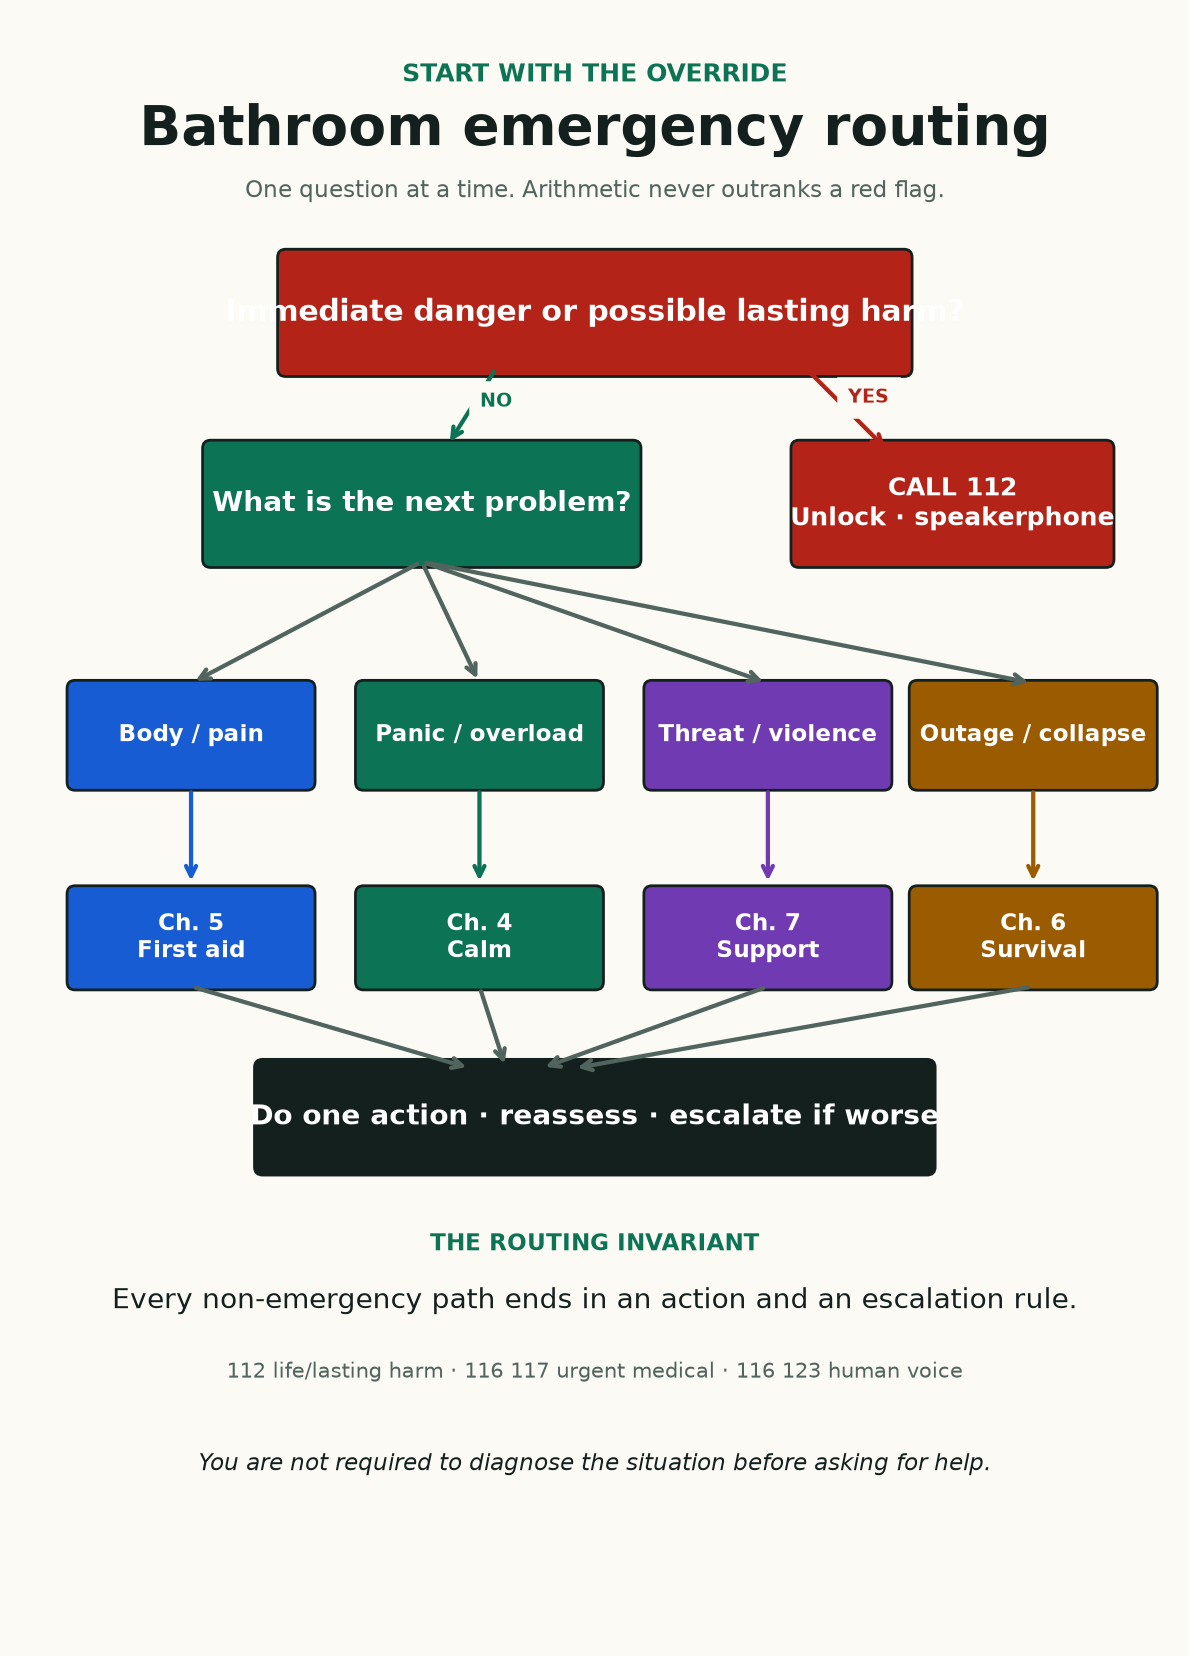
\includegraphics{build/diagrams/emergency_flowgraph.png}
\caption{Red-flag-first emergency decision flowgraph}
\end{figure}

\hypertarget{four-routes}{%
\subsection{Four routes}\label{four-routes}}

Red flag

Call 112. Then do only what the dispatcher asks and what is safe.

Body / pain

Go to Ch.5. Start with red flags, then simple first aid.

Panic / overload

Go to Ch.4. Orient outward, slow down, choose one action.

Threat / responsibility

Go to Ch.2 or Ch.7. Safety first; repair comes after stabilization.

Outage / collapse

Go to Ch.6. Verify the hazard, conserve resources, coordinate.

\hypertarget{the-seven-doors-into-the-guide}{%
\subsection{The seven doors into the
guide}\label{the-seven-doors-into-the-guide}}

\begin{longtable}[]{@{}lll@{}}
\toprule\noalign{}
Door & What is happening & First destination \\
\midrule\noalign{}
\endhead
\bottomrule\noalign{}
\endlastfoot
A & I caused trouble or someone depends on me & Ch.2 Responsibility \\
B & I feel anxious, panicky, or unreal & Ch.4 Calm \\
C & I feel pain or physically unwell & Ch.5 First aid \\
D & I feel endangered & Ch.7 Safety and support \\
E & Everything is congesting & Ch.4 Calm, then one task \\
F & There is a bad or unknown smell & Ch.3F Safety check \\
G & I have no place to go & Ch.7 Practical support \\
\end{longtable}

Several doors may be open. Red flags outrank all of them.

\hypertarget{basic-theorem-1-red-flag-dominance}{%
\subsection{Basic theorem 1 --- red-flag
dominance}\label{basic-theorem-1-red-flag-dominance}}

Let each red flag be a Boolean value \(r_i \in \{0,1\}\):

\[R = r_1 \lor r_2 \lor \cdots \lor r_n\]

If \(R=1\), the route is \textbf{112}. No anxiety score, pain score,
formula, or bathroom philosophy may cancel that result. This is a
routing rule, not a medical model.

\hypertarget{basic-theorem-2-the-one-next-action-rule}{%
\subsection{Basic theorem 2 --- the one-next-action
rule}\label{basic-theorem-2-the-one-next-action-rule}}

Acute stress reduces the amount of information people can reliably hold
and use. The guide therefore keeps a tiny queue:

\[Q = [\text{one action},\; \text{one backup},\; \text{one escalation rule}]\]

Example: \textbf{sit down → call a friend → if chest pain or fainting
appears, call 112}. A plan with twelve beautiful steps is decorative. A
plan with one executable step is equipment.\footnote{World Health
  Organization, \emph{Doing What Matters in Times of Stress} (2020):
  https://www.who.int/publications/i/item/9789240003927}

\hypertarget{reassessment-loop}{%
\subsection{Reassessment loop}\label{reassessment-loop}}

\begin{enumerate}
\def\labelenumi{\arabic{enumi}.}
\tightlist
\item
  \textbf{Act:} do the smallest safe action.
\item
  \textbf{Check:} better, same, or worse?
\item
  \textbf{Escalate:} if worse, new red flags appear, or uncertainty
  remains.
\item
  \textbf{Repeat:} only while the situation remains non-emergent.
\end{enumerate}

This is the guide's only intentional loop. It prevents both frozen
inaction and heroic improvisation.

\hypertarget{02-situation-a}{}
\hypertarget{situation-a-i-caused-trouble}{%
\section{Situation A --- I Caused
Trouble}\label{situation-a-i-caused-trouble}}

Guilt wants a trial. Emergencies need a sequence.

\hypertarget{first-split-live-problem-or-aftermath}{%
\subsection{First split: live problem or
aftermath?}\label{first-split-live-problem-or-aftermath}}

\hypertarget{a-live-problem}{%
\subsubsection{A live problem}\label{a-live-problem}}

If a person is injured, unresponsive, not breathing normally, bleeding
heavily, giving birth unexpectedly, or at risk of lasting harm:

\begin{enumerate}
\def\labelenumi{\arabic{enumi}.}
\tightlist
\item
  Call \textbf{112}.
\item
  Make the scene safe without creating a second casualty.
\item
  Follow Ch.5 and the dispatcher.
\item
  Do not spend the useful minutes deciding whose fault it is.
\end{enumerate}

If violence is active, leave the immediate danger if you safely can.
Call \textbf{110} for police; call \textbf{112} for medical rescue or
when immediate danger to life exists.

\hypertarget{the-aftermath}{%
\subsubsection{The aftermath}\label{the-aftermath}}

When nobody is in immediate danger, use the repair sequence:

\[A = (\text{stop},\; \text{stabilize},\; \text{tell},\; \text{repair},\; \text{follow up})\]

\begin{itemize}
\tightlist
\item
  \textbf{Stop:} stop the harmful action or process.
\item
  \textbf{Stabilize:} prevent further harm.
\item
  \textbf{Tell:} inform the affected person or responsible professional
  plainly.
\item
  \textbf{Repair:} replace, compensate, apologize, document, or obtain
  care.
\item
  \textbf{Follow up:} check whether the repair worked.
\end{itemize}

This is not absolution algebra. It is simply harder for shame to
sabotage five verbs than one enormous moral fog.

\hypertarget{pregnancy-birth-and-reproductive-decisions}{%
\subsection{Pregnancy, birth, and reproductive
decisions}\label{pregnancy-birth-and-reproductive-decisions}}

A pregnancy is not a flowchart puzzle and viability statistics do not
decide a person's values.

\begin{itemize}
\tightlist
\item
  \textbf{Unexpected active birth, heavy bleeding, seizure, fainting,
  severe pain, severe breathlessness, or serious concern:} call
  \textbf{112}.
\item
  \textbf{Urgent but not life-threatening symptoms:} contact maternity
  care, a gynecological service, or \textbf{116 117} outside practice
  hours.
\item
  \textbf{Decision or conflict about a pregnancy:} use a recognized
  pregnancy counselling service. A calm, confidential appointment is
  more useful than a milestone table copied into a bathroom.
\item
  \textbf{Medication exposure during pregnancy:} contact a clinician or
  a specialist service such as Embryotox; do not stop prescribed
  medication solely because of this guide.
\end{itemize}

If a baby has just arrived unexpectedly, keep parent and baby warm, do
not pull on the cord, call \textbf{112}, and follow the dispatcher's
instructions. Clever improvisation has been officially cancelled.

\hypertarget{child-dependent-adult-animal-or-other-responsibility}{%
\subsection{Child, dependent adult, animal, or other
responsibility}\label{child-dependent-adult-animal-or-other-responsibility}}

Ask four concrete questions:

\begin{longtable}[]{@{}
  >{\raggedright\arraybackslash}p{(\columnwidth - 4\tabcolsep) * \real{0.3333}}
  >{\raggedright\arraybackslash}p{(\columnwidth - 4\tabcolsep) * \real{0.3333}}
  >{\raggedright\arraybackslash}p{(\columnwidth - 4\tabcolsep) * \real{0.3333}}@{}}
\toprule\noalign{}
\begin{minipage}[b]{\linewidth}\raggedright
Question
\end{minipage} & \begin{minipage}[b]{\linewidth}\raggedright
If yes
\end{minipage} & \begin{minipage}[b]{\linewidth}\raggedright
If no
\end{minipage} \\
\midrule\noalign{}
\endhead
\bottomrule\noalign{}
\endlastfoot
Is anyone unsafe now? & 112 / 110 / veterinary emergency & Continue \\
Is essential care missing today? & Arrange food, medication,
supervision, shelter & Continue \\
Is this beyond one person's capacity? & Call family, care service, youth
office, vet, or crisis support & Continue \\
Is exhaustion making aggression feel possible? & Create distance safely
and get immediate support & Make a follow-up plan \\
\end{longtable}

Caregiver strain is not a character defect. It is a load problem. Load
problems need relief, rotation, and services---not more private
heroism.\footnote{gesund.bund.de, ``Überlastung bei pflegenden
  Angehörigen'' (updated 2025), including crisis and relief options:
  https://gesund.bund.de/belastungen-pflegende-angehoerige}

\hypertarget{harmed-someone}{%
\subsection{Harmed someone}\label{harmed-someone}}

\begin{itemize}
\tightlist
\item
  \textbf{Accident:} stabilize, get medical help, preserve facts, and
  report what happened honestly.
\item
  \textbf{Anger or loss of control:} create distance, remove access to
  weapons or dangerous objects if safe, and contact crisis or
  professional support.
\item
  \textbf{Self-defence or coercion:} get safe and obtain legal advice;
  do not rely on a paragraph summary of German criminal law.
\item
  \textbf{Thoughts of harming yourself or another person:} do not stay
  alone with the means to act. Call \textbf{112} for acute danger, or
  \textbf{116 123 / 116 117} for immediate support when there is no
  acute danger.
\end{itemize}

\hypertarget{a-silicon-based-life-form-escaped}{%
\subsection{A silicon-based life form
escaped}\label{a-silicon-based-life-form-escaped}}

Fine. The guide accepts one science-fiction branch.

\begin{enumerate}
\def\labelenumi{\arabic{enumi}.}
\tightlist
\item
  Disconnect or isolate the affected system if authorized and safe.
\item
  Do not wipe it, ``test one more thing,'' or publish credentials.
\item
  Preserve logs and timestamps.
\item
  Notify the system owner or incident-response contact.
\item
  If critical infrastructure or a serious cyber incident is involved,
  consult BSI guidance.
\end{enumerate}

Contain first. Post-mortem later. The server does not need your guilt,
only its logs.

\hypertarget{accountability-theorem}{%
\subsection{Accountability theorem}\label{accountability-theorem}}

Self-punishment and repair are not the same variable:

\[\text{remorse} \neq \text{repair}\]

Useful accountability increases truth, safety, and restitution. If an
action only increases your suffering while changing nothing for the
affected party, it may be punishment---but it is not yet repair.

\hypertarget{03-situations-b-g}{}
\hypertarget{situations-bg-pick-the-closest-door}{%
\section{Situations B--G --- Pick the Closest
Door}\label{situations-bg-pick-the-closest-door}}

\hypertarget{b-i-feel-anxious}{%
\subsection{B --- I feel anxious}\label{b-i-feel-anxious}}

First, check the override: new chest pressure, severe breathlessness,
fainting, one-sided weakness, confusion, a seizure, or a feeling that
this may be a medical emergency means \textbf{112}, not ``probably
anxiety.''

If no red flag is present:

\begin{enumerate}
\def\labelenumi{\arabic{enumi}.}
\tightlist
\item
  Put both feet on the floor or sit safely.
\item
  Name five things you can see and three sounds you can hear.
\item
  Let the exhale be gentle and slightly longer than the inhale.
\item
  Text or call one person: ``I am overloaded. Stay with me for ten
  minutes.''
\item
  Continue with Ch.4.
\end{enumerate}

The \textbf{GAD-7} asks about symptoms over the last \textbf{two weeks}.
It can support a conversation with a clinician; it is not an acute panic
triage score and it cannot rule out a physical emergency.\footnote{Spitzer
  RL et al., ``A Brief Measure for Assessing Generalized Anxiety
  Disorder: The GAD-7,'' \emph{Archives of Internal Medicine} 166
  (2006): 1092--1097. https://doi.org/10.1001/archinte.166.10.1092}

\hypertarget{c-i-feel-pain}{%
\subsection{C --- I feel pain}\label{c-i-feel-pain}}

Pain scores describe experience; they do not measure tissue damage,
blood loss, or urgency.

You may use a 0--10 number to communicate change:

\[\Delta P = P_{now} - P_{earlier}\]

That difference is useful for a conversation. It is not a diagnosis.
Sudden severe pain, chest pain, severe abdominal pain, new neurological
symptoms, major injury, pregnancy-related red flags, or pain with
collapse routes to \textbf{112}. Otherwise continue with Ch.5 or
\textbf{116 117}.

\hypertarget{d-i-feel-endangered}{%
\subsection{D --- I feel endangered}\label{d-i-feel-endangered}}

\hypertarget{danger-is-present-now}{%
\subsubsection{Danger is present now}\label{danger-is-present-now}}

\begin{itemize}
\tightlist
\item
  Move toward an exit, other people, or a lockable safe
  place---whichever reduces danger rather than trapping you.
\item
  Keep noise and screen light low if discovery creates risk.
\item
  Call \textbf{110} for police. Call \textbf{112} for medical rescue or
  immediate danger to life.
\item
  Do not confront the person to obtain a cleaner narrative.
\end{itemize}

\hypertarget{the-danger-is-a-memory-message-or-expected-encounter}{%
\subsubsection{The danger is a memory, message, or expected
encounter}\label{the-danger-is-a-memory-message-or-expected-encounter}}

Save messages and timestamps, tell one trusted person, plan transport
and a place to stay, and contact a specialist service. The Germany-wide
Violence against Women Helpline is \textbf{116 016}, anonymous, free,
multilingual, and available around the clock.\footnote{Federal Violence
  against Women Helpline, official service information:
  https://www.hilfetelefon.de/}

\hypertarget{e-things-are-congesting}{%
\subsection{E --- Things are congesting}\label{e-things-are-congesting}}

Overload often feels like every task became urgent at once. They did
not.

Write three lines:

\begin{enumerate}
\def\labelenumi{\arabic{enumi}.}
\tightlist
\item
  \textbf{Must prevent harm today}
\item
  \textbf{Must happen soon}
\item
  \textbf{Can survive being ugly}
\end{enumerate}

Now choose one action under five minutes. The rest goes on paper, not in
working memory.

A useful capacity model is:

\[L = I + E + S\]

where \(I\) is intrinsic task difficulty, \(E\) is avoidable clutter,
and \(S\) is stress load. You may not be able to reduce \(I\)
immediately, but closing tabs, silencing notifications, sitting down, or
asking someone else to hold a task reduces \(E\) or \(S\).\footnote{Cowan
  N, ``The magical number 4 in short-term memory,'' \emph{Behavioral and
  Brain Sciences} 24 (2001): 87--114. The estimate concerns controlled
  laboratory tasks and is a design clue, not a fixed personal limit.
  https://doi.org/10.1017/S0140525X01003922}

\hypertarget{f-bad-smell}{%
\subsection{F --- Bad smell}\label{f-bad-smell}}

Do \textbf{not} light a match to diagnose or ``neutralize'' an unknown
smell.

\begin{itemize}
\tightlist
\item
  \textbf{Gas, solvent, burning plastic, chlorine, rotten-egg smell,
  dizziness, eye irritation, or headache:} do not operate electrical
  switches or create flames. Leave for fresh air, warn others, and call
  \textbf{112} from outside if poisoning or fire may be involved.
  Contact the utility or fire service as appropriate.
\item
  \textbf{Sewage smell:} ventilate if safe, run water into rarely used
  drains, and report a persistent problem to building management or a
  plumber.
\item
  \textbf{Ordinary bathroom smell:} ventilation, cleaning, and a closed
  toilet lid are acceptable technologies. Fire remains unnecessary.
\end{itemize}

Never mix household cleaners, especially chlorine bleach with acids or
ammonia.

\hypertarget{g-no-place-to-go}{%
\subsection{G --- No place to go}\label{g-no-place-to-go}}

``No place'' may mean no safe home, no room in a group, or no internal
place where thoughts stop shouting. The immediate question is practical:

\begin{itemize}
\tightlist
\item
  Where can you be safe for the next hour?
\item
  Who can know where you are?
\item
  What essential item must stay with you: medication, phone, charger,
  ID, keys?
\item
  Which service can help with tonight, not your entire biography?
\end{itemize}

For acute danger use \textbf{112 / 110}. For a psychological crisis
without acute danger use \textbf{116 123}, \textbf{116 117}, a local
crisis service, or a hospital psychiatric emergency department. For
housing insecurity, contact the local municipal emergency housing or
social service; Ch.7 has a call script.

\hypertarget{consolidated-route}{%
\subsection{Consolidated route}\label{consolidated-route}}

\begin{longtable}[]{@{}
  >{\raggedright\arraybackslash}p{(\columnwidth - 4\tabcolsep) * \real{0.3333}}
  >{\raggedright\arraybackslash}p{(\columnwidth - 4\tabcolsep) * \real{0.3333}}
  >{\raggedright\arraybackslash}p{(\columnwidth - 4\tabcolsep) * \real{0.3333}}@{}}
\toprule\noalign{}
\begin{minipage}[b]{\linewidth}\raggedright
Situation
\end{minipage} & \begin{minipage}[b]{\linewidth}\raggedright
Do now
\end{minipage} & \begin{minipage}[b]{\linewidth}\raggedright
Escalate when
\end{minipage} \\
\midrule\noalign{}
\endhead
\bottomrule\noalign{}
\endlastfoot
Anxiety & Orient outward; contact one person & Red flag, self-harm risk,
or worsening \\
Pain & Check red flags; simple first aid & Sudden/severe/new
neurological or chest symptoms \\
Danger & Move to safety; call police/rescue & Threat is current or
injury exists \\
Congestion & Externalize; choose one action & Basic care or safety is
failing \\
Smell & No flame; leave unknown fumes & Fire, gas, chemical exposure,
symptoms \\
No place & Secure one hour; contact a service & Exposure, violence,
medical or self-harm risk \\
\end{longtable}

\hypertarget{04-calm-guide}{}
\hypertarget{calm-guide-reduce-the-volume-not-your-existence}{%
\section{Calm Guide --- Reduce the Volume, Not Your
Existence}\label{calm-guide-reduce-the-volume-not-your-existence}}

\hypertarget{before-calming-one-safety-check}{%
\subsection{Before calming: one safety
check}\label{before-calming-one-safety-check}}

If symptoms are new, severe, physically alarming, or unlike your usual
anxiety, use Ch.5 and call \textbf{112} when life or lasting harm may be
at risk. Calming is not a test you must pass before deserving medical
help.

\hypertarget{the-90-second-landing}{%
\subsection{The 90-second landing}\label{the-90-second-landing}}

\hypertarget{make-contact}{%
\subsubsection{1. Make contact}\label{make-contact}}

Sit or lean somewhere stable. Feel the floor, wall, or sink supporting
weight. Unclench the jaw. Drop the shoulders one centimetre---not
spiritually, literally.

\hypertarget{orient-outward}{%
\subsubsection{2. Orient outward}\label{orient-outward}}

Find:

\begin{itemize}
\tightlist
\item
  5 visible objects
\item
  4 contact points with your body
\item
  3 sounds
\item
  2 colours
\item
  1 next action
\end{itemize}

Grounding is an attention task. It need not produce enlightenment; it
only has to give the alarm system something ordinary to
process.\footnote{World Health Organization, \emph{Doing What Matters in
  Times of Stress} (2020):
  https://www.who.int/publications/i/item/9789240003927}

\hypertarget{breathe-comfortably}{%
\subsubsection{3. Breathe comfortably}\label{breathe-comfortably}}

Try a quiet inhale and a slightly longer, unforced exhale. No giant
gulps, no competition, no heroic breath-holding. Stop deliberate
breathing if it makes you dizzy, tingly, or more frightened and return
to normal breathing.

If inhale time is \(t_i\) and exhale time is \(t_e\), one cycle is

\[T = t_i + t_e, \qquad f = \frac{60}{T}\]

where \(f\) is breaths per minute. This formula describes pacing; it
does not prescribe one correct rate. Comfort and absence of dizziness
outrank the number.

\begin{figure}
\centering
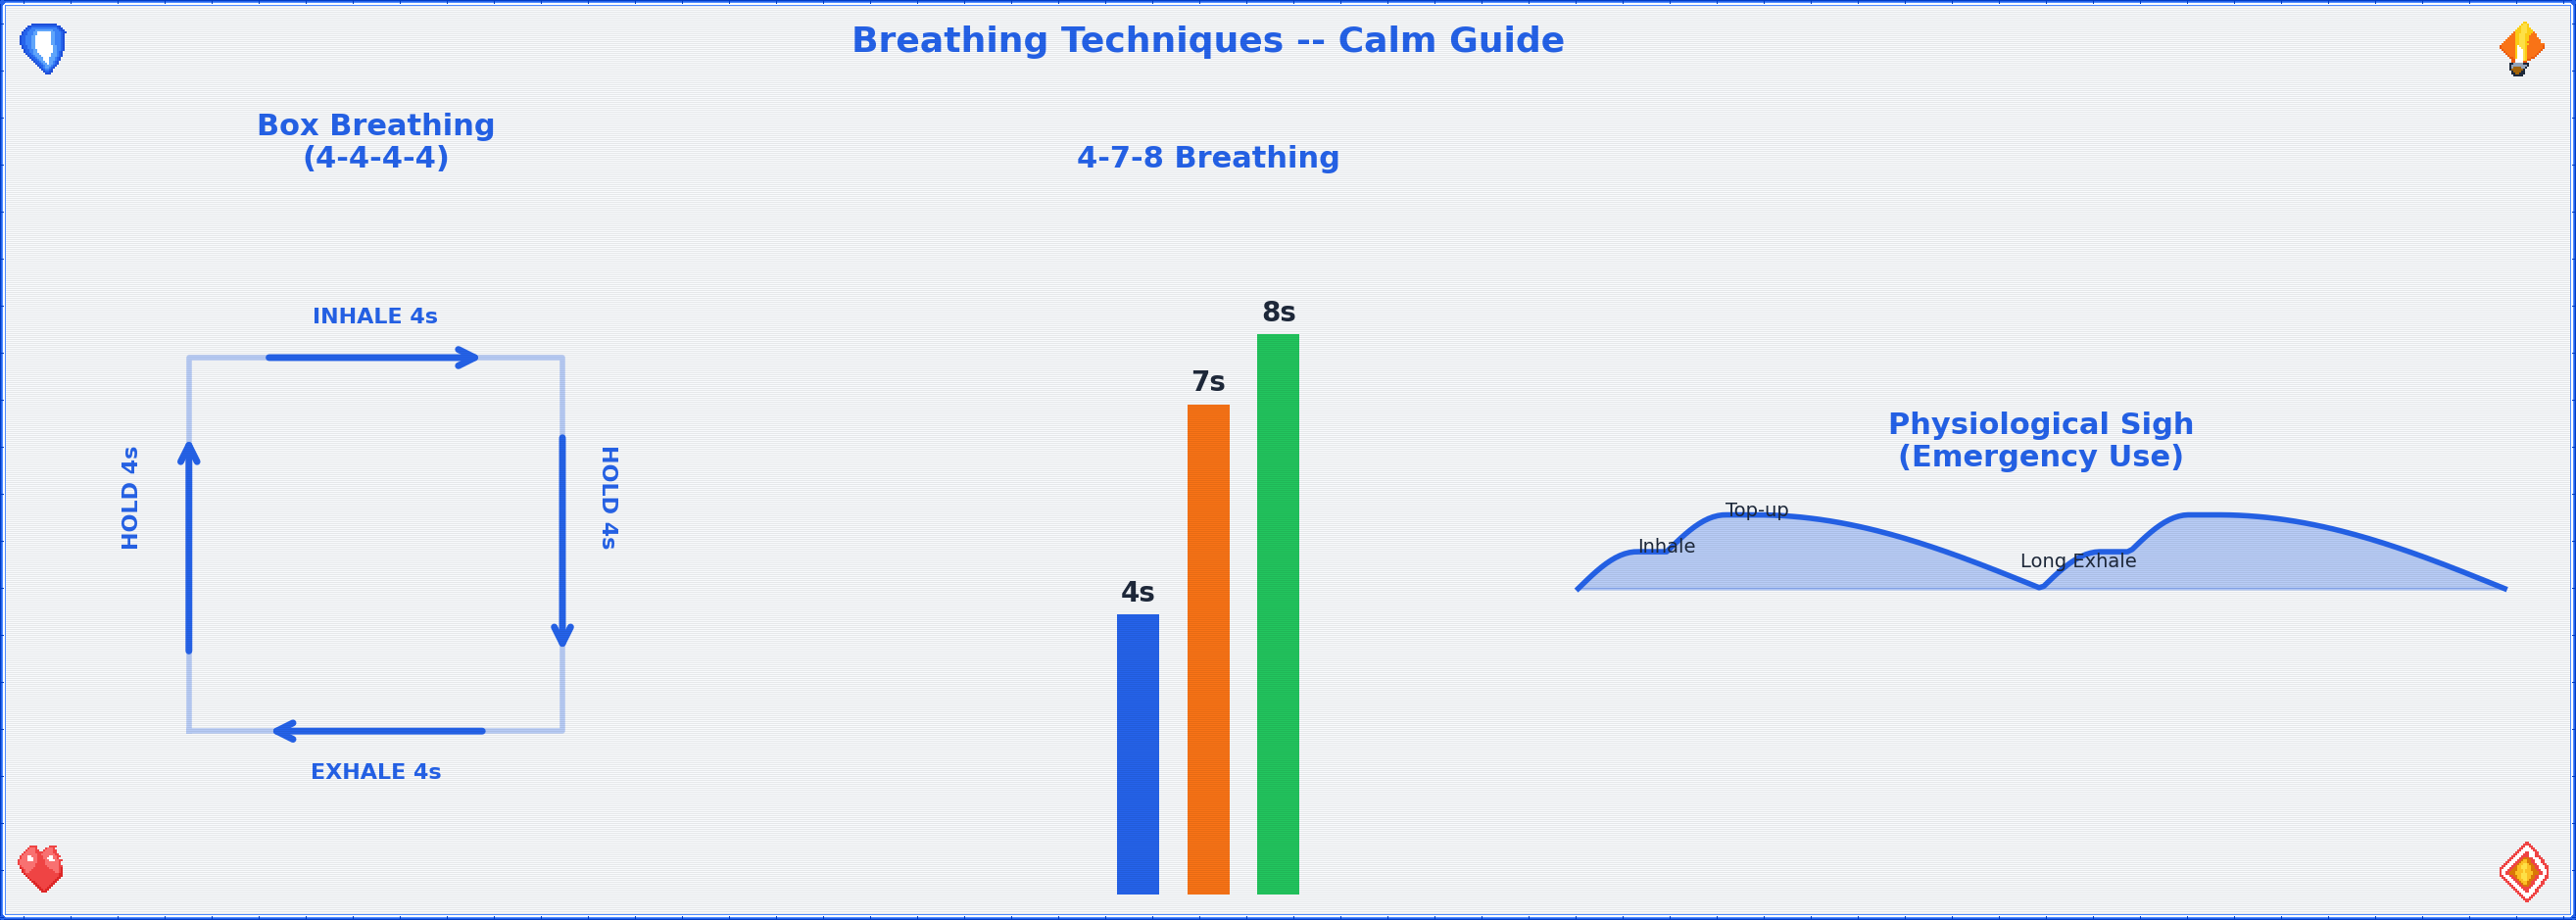
\includegraphics{build/diagrams/breathing_techniques.png}
\caption{Three optional breathing patterns}
\end{figure}

\hypertarget{a-small-menu-not-a-breathing-olympics}{%
\subsection{A small menu, not a breathing
Olympics}\label{a-small-menu-not-a-breathing-olympics}}

\hypertarget{longer-exhale}{%
\subsubsection{Longer exhale}\label{longer-exhale}}

Inhale gently for about 3 counts and exhale for about 4 or 5. Repeat
only while comfortable.

\hypertarget{physiological-sigh}{%
\subsubsection{Physiological sigh}\label{physiological-sigh}}

One inhale, a small second top-up inhale, then a long gentle exhale. One
to three repetitions may feel useful. A 2023 randomized study found that
five minutes of daily cyclic sighing over a month improved mood and
reduced respiratory rate; it did \textbf{not} prove that a single sigh
treats every acute panic episode.\footnote{Balban MY et al., ``Brief
  structured respiration practices enhance mood and reduce physiological
  arousal,'' \emph{Cell Reports Medicine} 4 (2023), 100895.
  https://doi.org/10.1016/j.xcrm.2022.100895}

\hypertarget{box-breathing}{%
\subsubsection{Box breathing}\label{box-breathing}}

Equal inhale, pause, exhale, pause can provide structure. Skip the
pauses if breath-holding feels bad or if a clinician has advised against
it.

The best technique is the one you can do without turning breathing into
another exam.

\hypertarget{the-bathroom-control-panel}{%
\subsection{The bathroom control
panel}\label{the-bathroom-control-panel}}

Check the boring variables:

\begin{longtable}[]{@{}
  >{\raggedright\arraybackslash}p{(\columnwidth - 2\tabcolsep) * \real{0.5000}}
  >{\raggedright\arraybackslash}p{(\columnwidth - 2\tabcolsep) * \real{0.5000}}@{}}
\toprule\noalign{}
\begin{minipage}[b]{\linewidth}\raggedright
Variable
\end{minipage} & \begin{minipage}[b]{\linewidth}\raggedright
Tiny correction
\end{minipage} \\
\midrule\noalign{}
\endhead
\bottomrule\noalign{}
\endlastfoot
Temperature & loosen clothing, cool or warm the room \\
Water & take a normal drink if thirsty and swallowing is safe \\
Blood sugar / food & eat something familiar if you have not eaten and
can do so safely \\
Noise / light & reduce one source \\
Medication & take only as prescribed; do not improvise doses \\
Contact & tell one person what is happening \\
Information & stop searching symptoms for ten minutes \\
\end{longtable}

\hypertarget{a-conceptual-calming-model}{%
\subsection{A conceptual calming
model}\label{a-conceptual-calming-model}}

Arousal does not have a universal exponential ``cortisol decay curve.''
Stress chemistry, attention, context, and safety interact. A more honest
model is a stepwise process:

\[A_{k+1} = A_k - \delta_k + \varepsilon_k\]

Here \(delta_k\) is the small reduction from a useful action and
\$arepsilon\_k\$ is whatever the world adds back. This is a teaching
model, not human physiology. The theorem is modest: several small
reductions can matter even when calm does not arrive in one cinematic
wave.

\hypertarget{unhook-from-the-thought}{%
\subsection{Unhook from the thought}\label{unhook-from-the-thought}}

Try the WHO phrasing:

\begin{quote}
``I notice the thought that \ldots{}''
\end{quote}

Not ``the thought is false,'' not ``I must defeat it.'' Just place one
grammatical layer between you and the sentence. Then ask: what action
fits the person I want to be for the next five minutes?

\hypertarget{leaving-the-bathroom}{%
\subsection{Leaving the bathroom}\label{leaving-the-bathroom}}

Use a three-line exit plan:

\begin{enumerate}
\def\labelenumi{\arabic{enumi}.}
\tightlist
\item
  \textbf{Destination:} ``I am going to the sofa / outside / to another
  person.''
\item
  \textbf{Sentence:} ``I got overloaded and needed a minute.''
\item
  \textbf{Backup:} ``If I spike again, I will step out and call X.''
\end{enumerate}

Open the door only when the next environment is safe. If the bathroom is
the safe place during violence, use Ch.3D and Ch.7 instead.

\hypertarget{when-calm-is-not-enough}{%
\subsection{When calm is not enough}\label{when-calm-is-not-enough}}

Seek professional help when episodes recur, avoidance grows, sleep or
daily function is deteriorating, substances are becoming the main coping
tool, or you are frightened of what you might do. Use \textbf{116 117}
for urgent non-life- threatening medical help, \textbf{116 123} for
crisis conversation, and \textbf{112} for acute self-harm or other
immediate danger.

\hypertarget{05-self-ambulance}{}
\hypertarget{first-aid-you-are-the-first-link-not-the-whole-ambulance}{%
\section{First Aid --- You Are the First Link, Not the Whole
Ambulance}\label{first-aid-you-are-the-first-link-not-the-whole-ambulance}}

This chapter is a prompt, not a first-aid qualification. Call
\textbf{112} early and follow the dispatcher. Put the phone on speaker.
Unlock the door if safe.

\hypertarget{the-first-minute}{%
\subsection{The first minute}\label{the-first-minute}}

\begin{enumerate}
\def\labelenumi{\arabic{enumi}.}
\tightlist
\item
  \textbf{Safety:} do not enter smoke, gas, traffic, electricity,
  violence, or chemical contamination.
\item
  \textbf{Response:} speak loudly and gently tap the shoulders.
\item
  \textbf{Call:} unresponsive, abnormal breathing, severe bleeding, or
  another red flag means \textbf{112}.
\item
  \textbf{Breathing:} look for normal breathing. Gasping is not normal
  breathing.
\item
  \textbf{Act:} use the matching section below.
\end{enumerate}

\begin{figure}
\centering
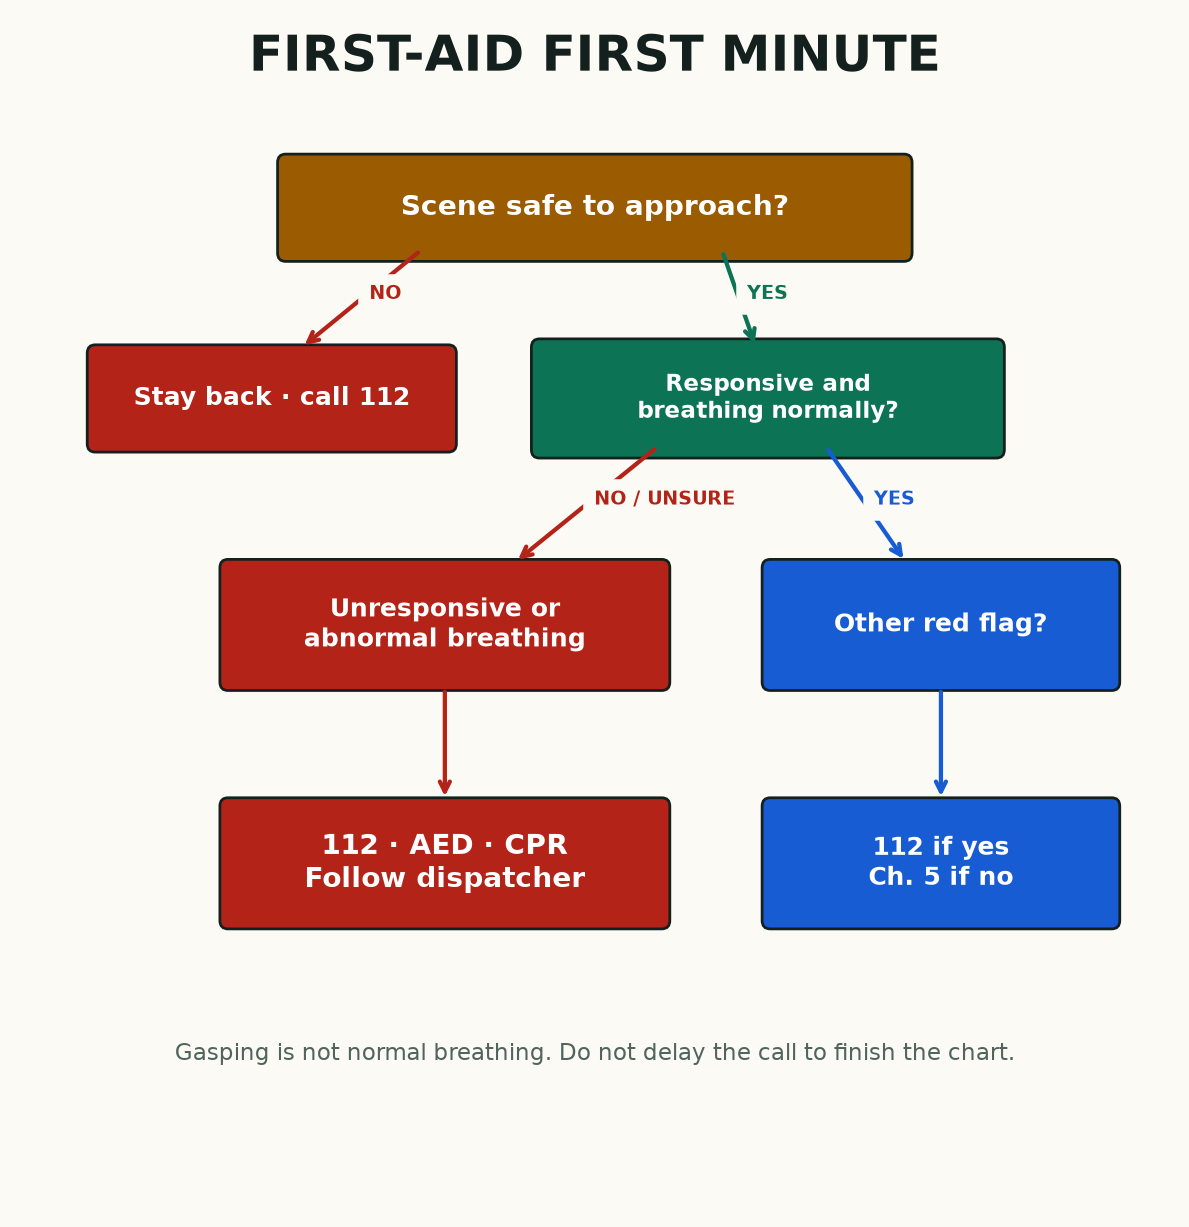
\includegraphics{build/diagrams/triage_flow.png}
\caption{First-aid triage overview}
\end{figure}

\hypertarget{unresponsive-and-not-breathing-normally}{%
\subsection{Unresponsive and not breathing
normally}\label{unresponsive-and-not-breathing-normally}}

\begin{itemize}
\tightlist
\item
  Call \textbf{112} and send someone for an AED if available.
\item
  Begin chest compressions in the centre of the adult chest:
  \textbf{100--120 per minute}, \textbf{5--6 cm} deep, allowing full
  recoil.
\item
  If trained and willing, use \textbf{30 compressions to 2 breaths}. If
  not, keep doing continuous chest compressions.
\item
  Switch rescuers when possible and use the AED as soon as it arrives.
\end{itemize}

The dispatcher can coach you. Imperfect compressions are better than
elegant inaction.\footnote{European Resuscitation Council,
  \emph{Guidelines 2025} and layperson guidance:
  https://www.erc.edu/science-research/guidelines/guidelines-2025/guidelines-2025-english/}

\hypertarget{unresponsive-but-breathing-normally}{%
\subsection{Unresponsive but breathing
normally}\label{unresponsive-but-breathing-normally}}

Call \textbf{112}, place the person in the recovery position if no major
trauma prevents safe movement, and keep checking breathing. Do not give
food or drink. If breathing becomes abnormal, start CPR.

\hypertarget{choking}{%
\subsection{Choking}\label{choking}}

If the person can cough effectively, encourage coughing. If they cannot
speak, breathe, or cough effectively, call \textbf{112} and follow the
dispatcher's choking instructions. If they become unresponsive, begin
CPR. Do not blindly sweep a finger inside the mouth.

\hypertarget{severe-bleeding}{%
\subsection{Severe bleeding}\label{severe-bleeding}}

\begin{enumerate}
\def\labelenumi{\arabic{enumi}.}
\tightlist
\item
  Call \textbf{112}.
\item
  Press firmly and continuously on the wound with a dressing or clean
  cloth.
\item
  Keep the person warm and still.
\item
  If blood soaks through, maintain pressure and add material; do not
  repeatedly lift the first dressing to inspect your progress.
\item
  Leave embedded objects in place and press around them.
\end{enumerate}

A dispatcher may give additional instructions, including use of a
tourniquet when appropriate. Do not abandon direct pressure to search
for perfect gear.\footnote{German Red Cross, ``Starke Blutungen'':
  https://www.drk.de/hilfe-in-deutschland/erste-hilfe/blutungen-und-blutstillung/blutungen/}

\hypertarget{burns}{%
\subsection{Burns}\label{burns}}

\begin{itemize}
\tightlist
\item
  Stop the burning process and remove the person from danger.
\item
  Cool the affected area locally with gently running, lukewarm water for
  about \textbf{10 minutes}, stopping if the person becomes cold.
\item
  Remove jewellery or loose clothing near the burn, but not material
  stuck to skin.
\item
  Cover loosely with a clean non-fluffy dressing.
\item
  Do not use ice, butter, toothpaste, flour, creams, or burst blisters.
\item
  Call \textbf{112} for severe or extensive burns, breathing injury,
  electrical or chemical burns, facial burns with breathing risk, or any
  serious concern.
\end{itemize}

German Red Cross public guidance emphasizes local cooling without
causing hypothermia.\footnote{German Red Cross, public burn first-aid
  guidance:
  https://www.drk.de/hilfe-in-deutschland/erste-hilfe/erste-hilfe-handgriffe-fuer-den-sommer/}

\hypertarget{chemical-in-eye-or-on-skin}{%
\subsection{Chemical in eye or on
skin}\label{chemical-in-eye-or-on-skin}}

Protect yourself. Remove contaminated clothing if safe and flush
immediately with plenty of clean running water, directing runoff away
from unaffected skin. For eye exposure, hold lids open and remove
contact lenses only if easy. Call \textbf{112} for serious symptoms and
contact a poison centre for substance-specific advice.

\hypertarget{stroke-fast}{%
\subsection{Stroke --- FAST}\label{stroke-fast}}

\begin{itemize}
\tightlist
\item
  \textbf{F --- Face:} one side droops?
\item
  \textbf{A --- Arms:} one arm weak or drifting?
\item
  \textbf{S --- Speech:} slurred, strange, or absent?
\item
  \textbf{T --- Time:} call \textbf{112 immediately} and note when the
  person was last known well.
\end{itemize}

Do not wait for several signs. One sudden FAST sign is enough to call.

\hypertarget{chest-pain-or-severe-breathlessness}{%
\subsection{Chest pain or severe
breathlessness}\label{chest-pain-or-severe-breathlessness}}

Call \textbf{112} for strong chest pressure or pain, breathlessness,
cold sweat, collapse, pain spreading to arm/jaw/back, or serious
uncertainty. Let the person rest in the position that makes breathing
easiest. Do not drive yourself.

\hypertarget{anaphylaxis}{%
\subsection{Anaphylaxis}\label{anaphylaxis}}

Sudden breathing difficulty, throat or tongue swelling, collapse, or
rapidly progressing symptoms after an allergen is an emergency.

\begin{itemize}
\tightlist
\item
  Use the person's prescribed adrenaline auto-injector immediately
  according to its instructions.
\item
  Call \textbf{112}.
\item
  Keep them lying down unless breathing is easier sitting up; do not let
  them stand or walk.
\item
  Follow the dispatcher and device instructions for any further dose.
\end{itemize}

Antihistamines do not replace adrenaline in anaphylaxis.

\hypertarget{poisoning}{%
\subsection{Poisoning}\label{poisoning}}

\begin{itemize}
\tightlist
\item
  Acute collapse, breathing difficulty, seizure, severe symptoms, or
  possible life-threatening exposure: \textbf{112}.
\item
  Otherwise call a German poison information centre; gesund.bund.de
  maintains the official route and explains when to use 112.
\item
  Keep the package, label, plant, or a photo available.
\item
  Do \textbf{not} induce vomiting and do not give a home ``antidote''
  unless a poison specialist instructs you.
\item
  For inhaled fumes, protect yourself and move to fresh air only if this
  is safe.
\end{itemize}

\hypertarget{pain-without-a-red-flag}{%
\subsection{Pain without a red flag}\label{pain-without-a-red-flag}}

Record location, onset, what changed it, and a 0--10 rating if helpful.
A pain number is communication, not triage. Contact a practice or
\textbf{116 117} when the problem is urgent but not life-threatening,
especially if pain is new, persistent, worsening, or impairing
function.\footnote{Federal Ministry of Health portal, ``Nummern für den
  Notfall'' (updated 2025): https://gesund.bund.de/notfallnummern}

\hypertarget{while-waiting}{%
\subsection{While waiting}\label{while-waiting}}

\begin{itemize}
\tightlist
\item
  Keep the route to the door clear and pets contained.
\item
  Gather medication list, allergies, ID, and the time symptoms began.
\item
  Do not eat or drink if surgery, reduced consciousness, choking, or
  severe nausea may be relevant.
\item
  Recheck breathing and responsiveness.
\item
  If the condition changes, tell the dispatcher.
\end{itemize}

\hypertarget{red-flag-theorem-again}{%
\subsection{Red-flag theorem, again}\label{red-flag-theorem-again}}

\[R=1 \Rightarrow \text{call 112}\]

Vital signs, pain scores, internet searches, and apparent calm can add
information. None of them reliably cancel a red flag for a lay reader.

\hypertarget{06-zombie-guide}{}
\hypertarget{zombie-guide-mostly-for-non-zombie-disasters}{%
\section{Zombie Guide --- Mostly for Non-Zombie
Disasters}\label{zombie-guide-mostly-for-non-zombie-disasters}}

No confirmed zombie outbreak is known. Power cuts, floods, heat,
contaminated water, smoke, and communication failures are real enough.
The fictional label stays because a guide is more likely to be read when
it contains one zombie.

\hypertarget{verify-before-optimizing}{%
\subsection{Verify before optimizing}\label{verify-before-optimizing}}

\begin{enumerate}
\def\labelenumi{\arabic{enumi}.}
\tightlist
\item
  Check official warnings: \textbf{NINA}, Cell Broadcast, local radio,
  municipality, police, fire service, or BBK.
\item
  Identify the hazard: fire, flood, chemical release, outage, violence,
  or ordinary rumour wearing tactical trousers.
\item
  Decide whether authorities say \textbf{shelter} or \textbf{evacuate}.
\item
  Tell one other person what you know and where you are.
\end{enumerate}

Do not leave a safe building merely because a group chat has cinematic
energy.

\hypertarget{survival-mathematics-model-not-prophecy}{%
\subsection{Survival mathematics --- model, not
prophecy}\label{survival-mathematics-model-not-prophecy}}

A standard survival function can be written as

\[S(t)=\exp\left(-\int_0^t h(u)\,du\right)\]

where \(h(u)\) is a hazard rate. Without measured hazards this formula
predicts nothing. Its practical lesson is simpler: reduce known
hazards---smoke exposure, unsafe water, cold, isolation---rather than
inventing a percentage for survival.

\begin{figure}
\centering
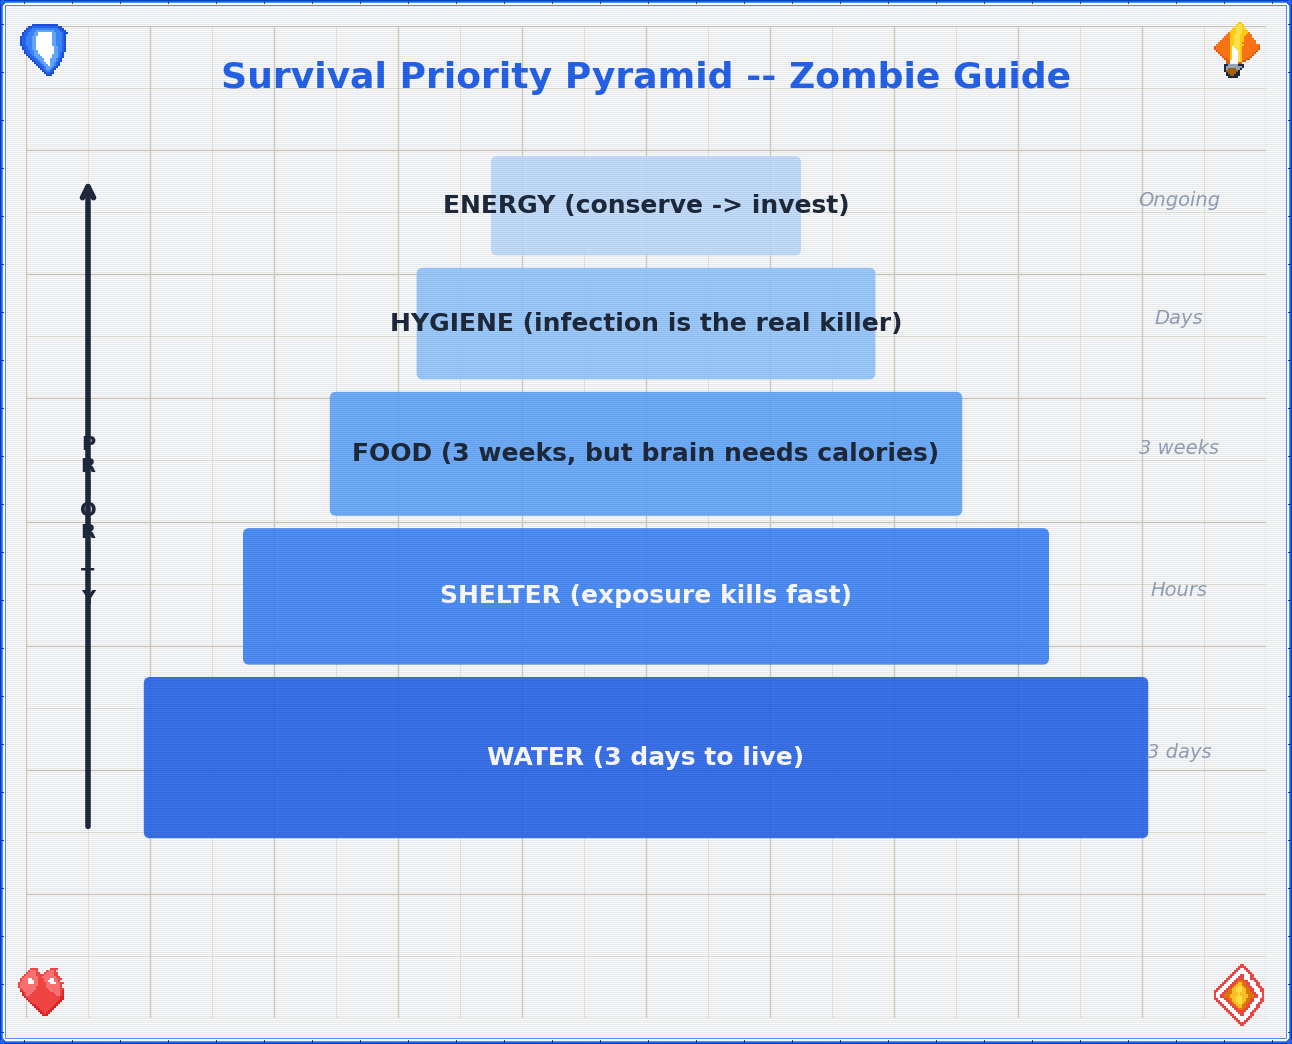
\includegraphics{build/diagrams/survival_pyramid.png}
\caption{Priority pyramid for disrupted infrastructure}
\end{figure}

\hypertarget{water}{%
\subsection{Water}\label{water}}

For household emergency storage, the 2025 BBK guide recommends ideally
\textbf{2 litres per person per day}, including about 0.5 L for cooking.
For \(n\) people over \(d\) days:

\[W = 2nd\;\text{litres}\]

Add pet needs. Heat, illness, pregnancy, breastfeeding, and physical
work can increase requirements. Follow local water advisories.

\begin{itemize}
\tightlist
\item
  Store potable water in clean, food-safe containers.
\item
  If authorities issue a boil-water notice, follow its exact
  instructions.
\item
  Filtering cloudy water through cloth may remove particles; it does not
  make microbiologically or chemically unsafe water safe.
\item
  Do not use a generic ``drops of bleach'' recipe: products and
  concentrations differ.
\item
  Water contaminated by fuel, solvents, pesticides, or radioactive
  material is not made safe by boiling.\footnote{Bundesamt für
    Bevölkerungsschutz und Katastrophenhilfe, \emph{Vorsorgen für Krisen
    und Katastrophen} (2025), especially the water and individual-needs
    checklists:
    https://www.bbk.bund.de/SharedDocs/Downloads/DE/Mediathek/Publikationen/Buergerinformationen/Ratgeber/BBK-Vorsorgen-fuer-Krisen-und-Katastrophen.pdf?\_\_blob=publicationFile\&v=44}
\end{itemize}

\hypertarget{air-fire-and-carbon-monoxide}{%
\subsection{Air, fire, and carbon
monoxide}\label{air-fire-and-carbon-monoxide}}

Never run generators, charcoal grills, camping stoves, or open flames
inside a home, garage, cellar, tent, or bathroom. Carbon monoxide is
colourless and odourless. Move to fresh air and call \textbf{112} if
poisoning is suspected.

Unknown gas or chemical smell means no matches and no electrical
switches. Leave if safe and call from outside.

\hypertarget{food-and-medication}{%
\subsection{Food and medication}\label{food-and-medication}}

\begin{itemize}
\tightlist
\item
  Use refrigerated food first while it is still safe.
\item
  Keep fridge and freezer doors closed during outages.
\item
  Discard food when official safety guidance or obvious spoilage says
  so; smell alone cannot detect every hazard.
\item
  Keep a medication list and a reasonable reserve agreed with the
  prescriber or pharmacy. Protect medicines requiring refrigeration.
\item
  Do not forage from a four-item list in an emergency guide.
  Misidentification is a terrible side quest.
\end{itemize}

\hypertarget{hygiene}{%
\subsection{Hygiene}\label{hygiene}}

Reserve clean water for drinking and essential food preparation. Use
separate containers for drinking and washing. Keep hands clean after
toilet use and before food handling. If toilets fail, follow municipal
sanitation guidance; contain waste away from food and water.

\hypertarget{power-and-information}{%
\subsection{Power and information}\label{power-and-information}}

\begin{itemize}
\tightlist
\item
  Charge phones and power banks while power exists.
\item
  Use battery radio and official alerts.
\item
  Keep one paper list of contacts, medications, and meeting points.
\item
  Send concise texts; networks often carry text when voice calls fail.
\item
  Preserve battery by lowering brightness and disabling unnecessary
  radios.
\end{itemize}

\hypertarget{group-coordination}{%
\subsection{Group coordination}\label{group-coordination}}

A fully connected group of \(n\) people has

\[C(n)=\frac{n(n-1)}{2}\]

possible pairwise communication channels. At \(n=10\), that is 45
channels; at \(n=30\), 435. The exact formula explains why ``everyone
tells everyone'' collapses quickly.

Use roles and a short briefing:

\begin{itemize}
\tightlist
\item
  safety and first aid
\item
  water and food
\item
  information and communications
\item
  care for children, disabled people, and animals
\item
  logistics and rest rotation
\end{itemize}

\begin{figure}
\centering
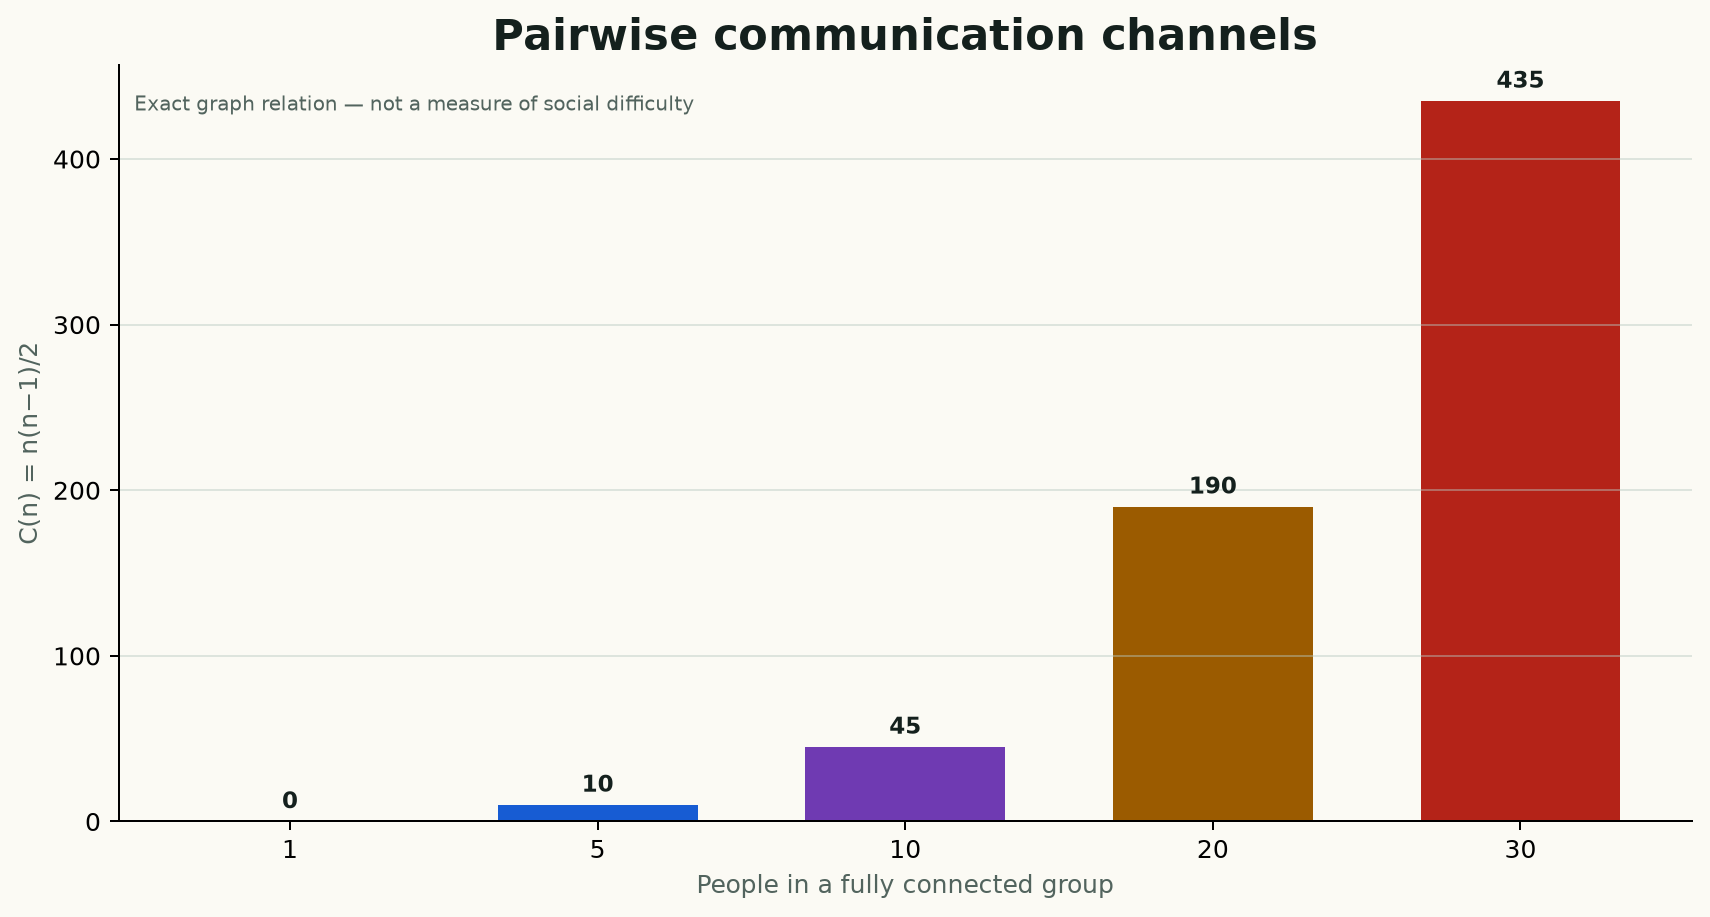
\includegraphics{build/diagrams/scaling_chart.png}
\caption{Coordination scaling from one person to a community}
\end{figure}

\hypertarget{commons-theorem}{%
\subsection{Commons theorem}\label{commons-theorem}}

Shared resources last longer when the group knows:

\begin{enumerate}
\def\labelenumi{\arabic{enumi}.}
\tightlist
\item
  what the resource is,
\item
  who may use it,
\item
  how use is recorded,
\item
  how rules can be changed,
\item
  how conflict is resolved.
\end{enumerate}

These echo Elinor Ostrom's empirically grounded design principles for
self-governed commons. They are not a magic constitution, but they beat
``the loudest person owns the water.''\footnote{Elinor Ostrom, ``Beyond
  Markets and States: Polycentric Governance of Complex Economic
  Systems,'' Nobel Prize Lecture (2009):
  https://www.nobelprize.org/prizes/economic-sciences/2009/ostrom/lecture/}

\hypertarget{evacuation-pocket-list}{%
\subsection{Evacuation pocket list}\label{evacuation-pocket-list}}

\begin{itemize}
\tightlist
\item
  phone + power bank
\item
  medication + medication list
\item
  ID, keys, payment method
\item
  water and simple food
\item
  weather layer / sturdy shoes
\item
  small first-aid kit
\item
  glasses, hearing aids, mobility supplies
\item
  infant, disability, and pet supplies
\item
  written destination and contact
\end{itemize}

Leave weapons, fantasies of looting, and twelve kilograms of
philosophical literature unless authorities specifically request an
ethics seminar.

\hypertarget{07-professional-support}{}
\hypertarget{professional-support-when-the-bathroom-is-too-small}{%
\section{Professional Support --- When the Bathroom Is Too
Small}\label{professional-support-when-the-bathroom-is-too-small}}

\hypertarget{germany-quick-reference}{%
\subsection{Germany quick reference}\label{germany-quick-reference}}

\begin{longtable}[]{@{}
  >{\raggedright\arraybackslash}p{(\columnwidth - 4\tabcolsep) * \real{0.3333}}
  >{\raggedright\arraybackslash}p{(\columnwidth - 4\tabcolsep) * \real{0.3333}}
  >{\raggedright\arraybackslash}p{(\columnwidth - 4\tabcolsep) * \real{0.3333}}@{}}
\toprule\noalign{}
\begin{minipage}[b]{\linewidth}\raggedright
Need
\end{minipage} & \begin{minipage}[b]{\linewidth}\raggedright
Contact
\end{minipage} & \begin{minipage}[b]{\linewidth}\raggedright
Use
\end{minipage} \\
\midrule\noalign{}
\endhead
\bottomrule\noalign{}
\endlastfoot
Life danger / possible lasting harm / fire & \textbf{112} & Rescue
service and fire brigade \\
Active crime or threat requiring police & \textbf{110} & Police \\
Urgent medical problem, not life-threatening & \textbf{116 117} &
Medical on-call service \\
Psychological crisis conversation & \textbf{116 123} & TelefonSeelsorge,
free and anonymous \\
Violence against women & \textbf{116 016} & 24/7, free, anonymous,
multilingual \\
Children and young people & \textbf{116 111} & Nummer gegen Kummer \\
Poisoning, no immediate life danger & regional poison centre & Directory
via gesund.bund.de \\
Immediate self- or other-endangerment & \textbf{112} & Rescue service \\
\end{longtable}

Numbers and scope were checked against the Federal Ministry of Health
portal and the official services on \textbf{17 July 2026}.\footnote{gesund.bund.de,
  ``Nummern für den Notfall'': https://gesund.bund.de/notfallnummern ;
  TelefonSeelsorge: https://www.telefonseelsorge.de/ ; Violence against
  Women Helpline: https://www.hilfetelefon.de/}

\hypertarget{the-call-script}{%
\subsection{The call script}\label{the-call-script}}

You do not need the right vocabulary. Use this:

\begin{quote}
``I am at \textbf{{[}address, floor, door code{]}}.\\
The problem is \textbf{{[}one sentence{]}}.\\
It started \textbf{{[}time{]}}.\\
The person is \textbf{{[}awake/unresponsive{]}} and \textbf{{[}breathing
normally/not{]}}.\\
There is \textbf{{[}danger/no known danger{]}} at the scene.\\
My callback number is \textbf{{[}number{]}}.''
\end{quote}

Then answer questions and stay on the line. Do not hang up merely
because the first sentence was delivered.

\hypertarget{psychological-crisis}{%
\subsection{Psychological crisis}\label{psychological-crisis}}

\hypertarget{acute-danger}{%
\subsubsection{Acute danger}\label{acute-danger}}

If someone may act on suicidal or violent thoughts, cannot stay safe, is
severely confused, or has lost contact with reality in a dangerous way,
call \textbf{112}. Stay nearby only if it is safe. Reduce access to
means if you can do so without confrontation or risk.

Asking directly ``Are you thinking about killing yourself?'' does not
plant the idea. It can clarify urgency. A ``yes,'' an unclear answer, or
inability to commit to immediate safety deserves real-time professional
help.

\hypertarget{urgent-support-without-acute-danger}{%
\subsubsection{Urgent support without acute
danger}\label{urgent-support-without-acute-danger}}

\begin{itemize}
\tightlist
\item
  \textbf{116 123} --- TelefonSeelsorge
\item
  \textbf{116 117} --- medical on-call service
\item
  local Sozialpsychiatrischer Dienst
\item
  psychiatric emergency department
\item
  GP or psychotherapist
\end{itemize}

The public health portal notes that local social psychiatric services
are free, accessible, may support relatives, and can sometimes make home
visits.\footnote{gesund.bund.de, ``Sozialpsychiatrischer Dienst -- Hilfe
  bei psychischen Krisen'' (2025):
  https://gesund.bund.de/sozialpsychiatrischer-dienst}

\hypertarget{violence-and-coercion}{%
\subsection{Violence and coercion}\label{violence-and-coercion}}

Do not optimize for a perfect confrontation. Optimize for safety.

\begin{itemize}
\tightlist
\item
  Use \textbf{110 / 112} during immediate danger.
\item
  \textbf{116 016} supports women affected by violence and people around
  them.
\item
  Save evidence only when doing so does not increase discovery risk.
\item
  Use a trusted device if the current device may be monitored.
\item
  Arrange a code word, transport, medication, documents, and a safe
  destination.
\end{itemize}

A bathroom lock is a delay mechanism, not a complete safety plan.

\hypertarget{medical-and-reproductive-support}{%
\subsection{Medical and reproductive
support}\label{medical-and-reproductive-support}}

\begin{itemize}
\tightlist
\item
  \textbf{112:} life danger or possible lasting harm.
\item
  \textbf{116 117:} urgent but not life-threatening problems outside
  practice hours.
\item
  GP / specialist / maternity service for ongoing assessment.
\item
  recognized pregnancy counselling for reproductive decisions.
\item
  Embryotox for evidence-based medication information in pregnancy and
  breastfeeding.
\end{itemize}

\hypertarget{children-dependants-and-caregiving}{%
\subsection{Children, dependants, and
caregiving}\label{children-dependants-and-caregiving}}

Contact pediatric or veterinary emergency services for acute health
problems. For care overload, involve family support, Pflegeberatung,
youth welfare, school, social services, or respite care before the
system relies on one exhausted person.

If you fear you may become aggressive, create safe distance, make sure
the dependent person is supervised, and call a crisis or emergency
service.

\hypertarget{housing-and-no-place-tonight}{%
\subsection{Housing and ``no place
tonight''}\label{housing-and-no-place-tonight}}

Call the local authority's emergency housing, social service, homeless
assistance, or an emergency shelter. Say:

\begin{quote}
``I have no safe place to sleep tonight. I am currently at
\textbf{{[}location{]}}. I have \textbf{{[}children / disability /
medication / pet / safety risk{]}}. Which service is responsible now,
and where can I go?''
\end{quote}

If exposure, violence, acute illness, or self-harm risk exists, use
\textbf{112 / 110}.

\hypertarget{fill-these-before-deployment}{%
\subsection{Fill these before
deployment}\label{fill-these-before-deployment}}

\begin{longtable}[]{@{}ll@{}}
\toprule\noalign{}
Local resource & Name / number \\
\midrule\noalign{}
\endhead
\bottomrule\noalign{}
\endlastfoot
Trusted person & \\
GP / practice & \\
Pharmacy & \\
Local crisis service & \\
Poison centre & \\
Safe place / shelter & \\
Building utility emergency & \\
Veterinary emergency & \\
\end{longtable}

\hypertarget{08-appendix}{}
\hypertarget{appendix-the-useful-loose-ends}{%
\section{Appendix --- The Useful Loose
Ends}\label{appendix-the-useful-loose-ends}}

\hypertarget{evidence-labels}{%
\subsection{Evidence labels}\label{evidence-labels}}

The guide now distinguishes three kinds of statement:

\begin{longtable}[]{@{}
  >{\raggedright\arraybackslash}p{(\columnwidth - 4\tabcolsep) * \real{0.3333}}
  >{\raggedright\arraybackslash}p{(\columnwidth - 4\tabcolsep) * \real{0.3333}}
  >{\raggedright\arraybackslash}p{(\columnwidth - 4\tabcolsep) * \real{0.3333}}@{}}
\toprule\noalign{}
\begin{minipage}[b]{\linewidth}\raggedright
Label
\end{minipage} & \begin{minipage}[b]{\linewidth}\raggedright
Meaning
\end{minipage} & \begin{minipage}[b]{\linewidth}\raggedright
Example
\end{minipage} \\
\midrule\noalign{}
\endhead
\bottomrule\noalign{}
\endlastfoot
\textbf{Protocol} & Action aligned with an authoritative guideline &
Call 112 for unresponsive abnormal breathing \\
\textbf{Descriptive equation} & Exact relation once inputs are known &
\(C(n)=n(n-1)/2\) \\
\textbf{Conceptual model} & A thinking aid, not a clinical prediction &
\(A_{k+1}=A_k-\delta_k+\varepsilon_k\) \\
\textbf{Mnemonic} & Memorable approximation & ``one action, one backup,
one escalation'' \\
\end{longtable}

The old edition sometimes dressed a metaphor in a lab coat. Version 4
makes the coat show its ID.

\hypertarget{formula-and-theorem-index}{%
\subsection{Formula and theorem index}\label{formula-and-theorem-index}}

\hypertarget{red-flag-dominance-routing-protocol}{%
\subsubsection{1. Red-flag dominance --- routing
protocol}\label{red-flag-dominance-routing-protocol}}

\[R = \bigvee_i r_i, \qquad R=1 \Rightarrow 112\]

A positive red flag overrides scores and self-reassurance.

\hypertarget{tiny-action-queue-design-theorem}{%
\subsubsection{2. Tiny action queue --- design
theorem}\label{tiny-action-queue-design-theorem}}

\[Q=[\text{action},\text{backup},\text{escalation}]\]

Acute instructions should fit in a small working-memory budget.

\hypertarget{pain-change-descriptive-communication}{%
\subsubsection{3. Pain change --- descriptive
communication}\label{pain-change-descriptive-communication}}

\[\Delta P=P_{now}-P_{earlier}\]

Useful for reporting change; not a measure of injury or urgency.

\hypertarget{breath-pacing-descriptive-equation}{%
\subsubsection{4. Breath pacing --- descriptive
equation}\label{breath-pacing-descriptive-equation}}

\[T=t_i+t_e, \qquad f=\frac{60}{T}\]

Describes a chosen pattern. Comfort and safety set the pattern.

\hypertarget{household-emergency-water-planning-equation}{%
\subsubsection{5. Household emergency water --- planning
equation}\label{household-emergency-water-planning-equation}}

\[W=2nd\;\text{litres}\]

BBK planning value for \(n\) people and \(d\) days; individual needs
vary.

\hypertarget{communication-channels-graph-theorem}{%
\subsubsection{6. Communication channels --- graph
theorem}\label{communication-channels-graph-theorem}}

\[C(n)=\frac{n(n-1)}{2}\]

Explains why groups need roles and broadcast channels.

\hypertarget{survival-function-mathematical-model}{%
\subsubsection{7. Survival function --- mathematical
model}\label{survival-function-mathematical-model}}

\[S(t)=\exp\left(-\int_0^t h(u)\,du\right)\]

Valid mathematics, useless as a personal forecast without measured
hazard data.

\hypertarget{accountability-tuple-procedural-mnemonic}{%
\subsubsection{8. Accountability tuple --- procedural
mnemonic}\label{accountability-tuple-procedural-mnemonic}}

\[A=(\text{stop},\text{stabilize},\text{tell},\text{repair},\text{follow up})\]

Turns guilt into observable repair work.

\hypertarget{pocket-print-card}{%
\subsection{Pocket print card}\label{pocket-print-card}}

RED FLAG?

112 · unlock if safe · speakerphone · follow dispatcher

Unresponsive · abnormal breathing · severe bleeding · stroke sign ·
chest pressure · severe breathlessness · seizure · major burn · collapse
· acute self/other danger

BODY

Ch.5 · first aid · 116 117 if urgent but non-life-threatening

ALARM

Feet · five objects · long gentle exhale · one person

THREAT

Exit / safer place · 110 · 116 016 · do not confront

OUTAGE

Official warning · water · air/fire · medication · roles

\hypertarget{offline-deployment-checklist}{%
\subsection{Offline deployment
checklist}\label{offline-deployment-checklist}}

\begin{itemize}
\tightlist
\item
  Print the monochrome PDF single-sided or duplex.
\item
  Write local contacts in Ch.7.
\item
  Keep the guide near a charged light source.
\item
  Add a simple first-aid poster from an official provider.
\item
  Refresh service numbers and medical guidance at each release.
\item
  Replace the guide after water damage. It is not itself waterproof,
  despite strong thematic alignment.
\end{itemize}

\hypertarget{navigation-invariant}{%
\subsection{Navigation invariant}\label{navigation-invariant}}

Every non-emergency route must provide:

\begin{enumerate}
\def\labelenumi{\arabic{enumi}.}
\tightlist
\item
  a next action,
\item
  a reason to escalate,
\item
  a named destination.
\end{enumerate}

A dead end in prose is still a dead end.

\hypertarget{09-version-history}{}
\hypertarget{version-history}{%
\section{Version History}\label{version-history}}

\hypertarget{july-2026}{%
\subsection{4.0.0 --- 17 July 2026}\label{july-2026}}

\hypertarget{technical-realization}{%
\subsubsection{Technical realization}\label{technical-realization}}

\begin{itemize}
\tightlist
\item
  Replaced CDN MathJax and timed browser waiting with native MathML.
\item
  Removed brittle cover-document CSS merging; chapters and cover now
  share one semantic document.
\item
  Added a Pandoc template with table of contents, mobile navigation,
  theme toggle, reading progress, and print action.
\item
  Rebuilt print CSS around an enforced A4 single-column invariant.
\item
  Added an independent monochrome layer without copying the full
  stylesheet.
\item
  Added Chrome and WeasyPrint PDF backends consuming identical HTML.
\item
  Added structural, safety-wording, MathML, image, A4, and page-count
  validation.
\item
  Fixed chapter assembly so repeated YAML frontmatter does not leak into
  output.
\end{itemize}

\hypertarget{orientation-and-ui}{%
\subsubsection{Orientation and UI}\label{orientation-and-ui}}

\begin{itemize}
\tightlist
\item
  Replaced route-first diagrams with a portrait, red-flag-first
  flowgraph.
\item
  Added four explicit destinations and a reassessment loop.
\item
  Reduced decorative cards and gradients in favour of a bathroom-tile,
  high-contrast utilitarian system.
\item
  Improved mobile contents navigation and print table/figure behaviour.
\end{itemize}

\hypertarget{content-and-evidence}{%
\subsubsection{Content and evidence}\label{content-and-evidence}}

\begin{itemize}
\tightlist
\item
  Corrected newborn/medical routing from 110 to 112.
\item
  Removed concentration-free bleach dosing, unsafe foraging advice,
  match-based smell advice, pain ``physiological correlates,'' and
  fictional cortisol decay.
\item
  Reframed GAD-7 and pain scales as communication/screening tools, not
  triage.
\item
  Rewrote CPR, bleeding, burn, stroke, poisoning, anaphylaxis, crisis,
  violence, water, outage, pregnancy, and caregiver sections against
  authoritative sources.
\item
  Marked every formula as protocol, descriptive equation, conceptual
  model, or mnemonic.
\item
  Expanded current German help numbers and source annotations.
\end{itemize}

\hypertarget{earlier-versions}{%
\subsection{Earlier versions}\label{earlier-versions}}

\begin{longtable}[]{@{}lll@{}}
\toprule\noalign{}
Version & Date & Summary \\
\midrule\noalign{}
\endhead
\bottomrule\noalign{}
\endlastfoot
3.4 & 2026-06-10 & experimental multi-backend and two-column work \\
3.2 & 2026-05-03 & formula and scientific-diagram expansion \\
3.0 & 2026-05-01 & modular content and source chapter \\
2.0 & 2026-04-29 & pixel assets and themed HTML/PDF \\
1.0 & 2026-04-29 & initial guide \\
\end{longtable}

Version 4 deliberately removes several ``scientific-looking'' claims
introduced in 3.2. More formulas are not automatically more science;
better boundaries are.

\hypertarget{10-sources}{}
\hypertarget{sources-and-evidence-notes}{%
\section{Sources and Evidence Notes}\label{sources-and-evidence-notes}}

Checked \textbf{17 July 2026}. Official and primary sources are
preferred. A link is not evidence by itself; the guide cites what each
source actually supports.

\hypertarget{emergency-routing-and-first-aid}{%
\subsection{Emergency routing and first
aid}\label{emergency-routing-and-first-aid}}

\begin{enumerate}
\def\labelenumi{\arabic{enumi}.}
\item
  \textbf{European Resuscitation Council --- Guidelines 2025.} Current
  European resuscitation framework, including adult basic life support,
  paediatric and newborn life support, and first aid.\\
  https://www.erc.edu/science-research/guidelines/guidelines-2025/guidelines-2025-english/
\item
  \textbf{ERC --- Guidelines 2025 for Everyone.} Lay version emphasizing
  early recognition, emergency activation, high-quality compressions,
  and AED use.\\
  https://www.erc.edu/media/p5ymaeej/gl2025\_layperson\_book\_ipdf-v11-e.pdf
\item
  \textbf{German Red Cross --- Finding a person in an emergency.} Scene
  safety, response and breathing checks, recovery position, emergency
  call, and CPR.\\
  https://www.drk.de/hilfe-in-deutschland/erste-hilfe/auffinden-einer-person/
\item
  \textbf{German Red Cross --- Severe bleeding.} Direct pressure,
  pressure dressing, warmth, monitoring, and 112 for life-threatening
  bleeding.\\
  https://www.drk.de/hilfe-in-deutschland/erste-hilfe/blutungen-und-blutstillung/blutungen/
\item
  \textbf{German Red Cross --- Public burn first aid.} Local lukewarm
  cooling, clean covering, avoidance of home remedies, and escalation
  for severe burns.\\
  https://www.drk.de/hilfe-in-deutschland/erste-hilfe/erste-hilfe-handgriffe-fuer-den-sommer/
\item
  \textbf{German Red Cross --- Chemical burns.} Self-protection, removal
  of contaminated clothing, and immediate irrigation.\\
  https://www.drk.de/hilfe-in-deutschland/erste-hilfe/veraetzungen/
\item
  \textbf{gesund.bund.de --- Emergency numbers.} Official German
  distinctions among 112, 116 117, poison centres, and crisis lines.\\
  https://gesund.bund.de/notfallnummern
\end{enumerate}

\hypertarget{psychological-crisis-and-calming}{%
\subsection{Psychological crisis and
calming}\label{psychological-crisis-and-calming}}

\begin{enumerate}
\def\labelenumi{\arabic{enumi}.}
\setcounter{enumi}{7}
\item
  \textbf{World Health Organization --- Doing What Matters in Times of
  Stress} (2020). Evidence-informed, field-tested grounding, unhooking,
  values, and small-action exercises.\\
  https://www.who.int/publications/i/item/9789240003927
\item
  \textbf{gesund.bund.de --- Managing psychological crises.} Safety
  escalation, professional help, social contact, and caution that
  inward-focused relaxation may intensify some acute crises.\\
  https://gesund.bund.de/mit-psychischen-krisen-umgehen
\item
  \textbf{Balban MY et al.} ``Brief structured respiration practices
  enhance mood and reduce physiological arousal.'' \emph{Cell Reports
  Medicine} 4 (2023),

  \begin{enumerate}
  \def\labelenumii{\arabic{enumii}.}
  \setcounter{enumii}{100894}
  \tightlist
  \item
    The trial studied five minutes of daily practice for 28 days; the
    guide avoids converting it into a universal one-breath emergency
    claim.\\
    https://doi.org/10.1016/j.xcrm.2022.100895
  \end{enumerate}
\item
  \textbf{Spitzer RL et al.} ``A Brief Measure for Assessing Generalized
  Anxiety Disorder: The GAD-7.'' \emph{Archives of Internal Medicine}
  166 (2006): 1092--1097. Supports a two-week symptom screen, not acute
  medical triage.\\
  https://doi.org/10.1001/archinte.166.10.1092
\item
  \textbf{Hjermstad MJ et al.} ``Studies comparing Numerical Rating
  Scales, Verbal Rating Scales, and Visual Analogue Scales for
  assessment of pain intensity in adults.'' \emph{Journal of Pain and
  Symptom Management} 41 (2011): 1073--1093. Supports pain intensity as
  patient report; not a stand-alone urgency score.\\
  https://pubmed.ncbi.nlm.nih.gov/21110961/
\item
  \textbf{Cowan N.} ``The magical number 4 in short-term memory.''
  \emph{Behavioral and Brain Sciences} 24 (2001): 87--114. Used as a
  design reason for short instructions, not a fixed capacity
  diagnosis.\\
  https://doi.org/10.1017/S0140525X01003922
\end{enumerate}

\hypertarget{german-crisis-and-support-services}{%
\subsection{German crisis and support
services}\label{german-crisis-and-support-services}}

\begin{enumerate}
\def\labelenumi{\arabic{enumi}.}
\setcounter{enumi}{13}
\item
  \textbf{TelefonSeelsorge.} Official free and anonymous crisis
  conversation: 116 123 and additional channels.\\
  https://www.telefonseelsorge.de/
\item
  \textbf{Violence against Women Helpline.} Official 116 016 service;
  free, anonymous, multilingual, 24/7.\\
  https://www.hilfetelefon.de/
\item
  \textbf{116117.de.} Official medical on-call service for urgent,
  non-life-threatening problems.\\
  https://www.116117.de/
\item
  \textbf{gesund.bund.de --- Social psychiatric service.} Public
  low-threshold support for people in crisis and their social
  environment.\\
  https://gesund.bund.de/sozialpsychiatrischer-dienst
\item
  \textbf{gesund.bund.de --- Caregiver overload.} Warning signs, relief,
  counselling, and acute-crisis options.\\
  https://gesund.bund.de/belastungen-pflegende-angehoerige
\item
  \textbf{Embryotox.} Evidence-based medication information and
  specialist counselling for pregnancy and breastfeeding.\\
  https://www.embryotox.de/
\item
  \textbf{familienplanung.de.} Federal public information and recognized
  pregnancy counselling search.\\
  https://www.familienplanung.de/beratung/beratungsstellensuche/
\end{enumerate}

\hypertarget{preparedness-water-and-groups}{%
\subsection{Preparedness, water, and
groups}\label{preparedness-water-and-groups}}

\begin{enumerate}
\def\labelenumi{\arabic{enumi}.}
\setcounter{enumi}{20}
\item
  \textbf{Bundesamt für Bevölkerungsschutz und Katastrophenhilfe.}
  \emph{Vorsorgen für Krisen und Katastrophen} (2025). Current German
  household preparedness, 2 L/person/day water planning value,
  individual needs, warnings, evacuation supplies, hygiene, and outage
  advice.\\
  https://www.bbk.bund.de/SharedDocs/Downloads/DE/Mediathek/Publikationen/Buergerinformationen/Ratgeber/BBK-Vorsorgen-fuer-Krisen-und-Katastrophen.pdf?\_\_blob=publicationFile\&v=44
\item
  \textbf{WHO --- Technical Notes on Drinking-Water, Sanitation and
  Hygiene in Emergencies.} Treatment guidance and the important limits
  of household methods.\\
  https://www.who.int/publications/m/item/technical-notes-on-drinking-water-sanitation-and-hygiene-in-emergencies
\item
  \textbf{Elinor Ostrom.} ``Beyond Markets and States: Polycentric
  Governance of Complex Economic Systems,'' Nobel Prize Lecture (2009).
  Empirical basis for commons-governance principles.\\
  https://www.nobelprize.org/prizes/economic-sciences/2009/ostrom/lecture/
\item
  \textbf{Inter-Agency Standing Committee.} \emph{Guidelines on Mental
  Health and Psychosocial Support in Emergency Settings.} Layered
  support from basic safety and services through specialized care.\\
  https://interagencystandingcommittee.org/iasc-task-force-mental-health-and-psychosocial-support-emergency-settings/iasc-guidelines-mental-health-and-psychosocial-support-emergency-settings-2007
\end{enumerate}

\hypertarget{cyber-incident-branch}{%
\subsection{Cyber incident branch}\label{cyber-incident-branch}}

\begin{enumerate}
\def\labelenumi{\arabic{enumi}.}
\setcounter{enumi}{24}
\tightlist
\item
  \textbf{Federal Office for Information Security (BSI).} Citizen and
  organizational incident information and reporting routes.\\
  https://www.bsi.bund.de/
\end{enumerate}

\hypertarget{editorial-policy}{%
\subsection{Editorial policy}\label{editorial-policy}}

\begin{itemize}
\tightlist
\item
  Do not infer acute medical urgency from a GAD-7 or pain score.
\item
  Do not print drug or chemical dosing without product- and
  concentration-specific authority.
\item
  Distinguish measured clinical relationships from explanatory models.
\item
  Prefer a short action plus escalation rule to an impressive but
  unusable lecture.
\item
  Recheck service numbers and guideline versions at every release.
\end{itemize}
